\documentclass{standalone}
\usepackage{tikz}
\usetikzlibrary{patterns, positioning}

\begin{document}
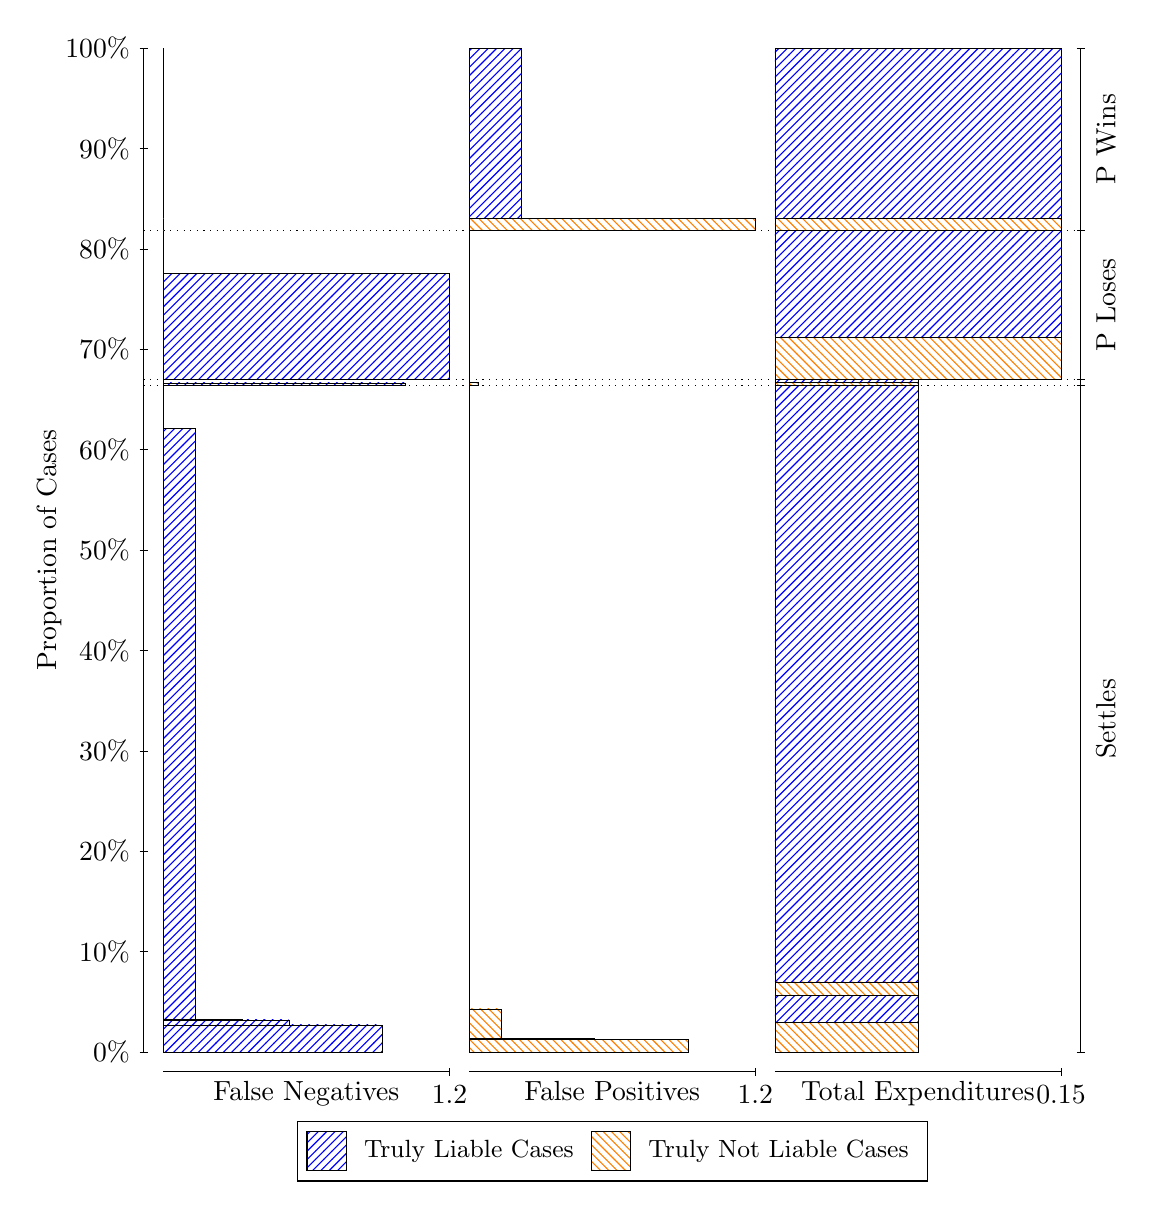
\begin{tikzpicture}
\draw[black, very thin] (1.5,1.75) -- (1.5,14.5);
\node[rotate=90, anchor=center] at (0.3, 8.125) {Proportion of Cases};
\draw[black, very thin] (1.45,1.75) -- (1.55,1.75);
\node[anchor=east] at (1.45, 1.75) {0\%};
\draw[black, very thin] (1.45,3.025) -- (1.55,3.025);
\node[anchor=east] at (1.45, 3.025) {10\%};
\draw[black, very thin] (1.45,4.3) -- (1.55,4.3);
\node[anchor=east] at (1.45, 4.3) {20\%};
\draw[black, very thin] (1.45,5.575) -- (1.55,5.575);
\node[anchor=east] at (1.45, 5.575) {30\%};
\draw[black, very thin] (1.45,6.85) -- (1.55,6.85);
\node[anchor=east] at (1.45, 6.85) {40\%};
\draw[black, very thin] (1.45,8.125) -- (1.55,8.125);
\node[anchor=east] at (1.45, 8.125) {50\%};
\draw[black, very thin] (1.45,9.4) -- (1.55,9.4);
\node[anchor=east] at (1.45, 9.4) {60\%};
\draw[black, very thin] (1.45,10.675) -- (1.55,10.675);
\node[anchor=east] at (1.45, 10.675) {70\%};
\draw[black, very thin] (1.45,11.95) -- (1.55,11.95);
\node[anchor=east] at (1.45, 11.95) {80\%};
\draw[black, very thin] (1.45,13.225) -- (1.55,13.225);
\node[anchor=east] at (1.45, 13.225) {90\%};
\draw[black, very thin] (1.45,14.5) -- (1.55,14.5);
\node[anchor=east] at (1.45, 14.5) {100\%};

\draw[black, very thin] (13.4,1.75) -- (13.4,14.5);
\draw[black, very thin] (13.35,1.75) -- (13.45,1.75);
\node[anchor=west] at (13.35, 1.75) {};
\draw[black, very thin] (13.35,10.212) -- (13.45,10.212);
\node[anchor=west] at (13.35, 10.212) {};
\draw[black, very thin] (13.35,10.287) -- (13.45,10.287);
\node[anchor=west] at (13.35, 10.287) {};
\draw[black, very thin] (13.35,12.182) -- (13.45,12.182);
\node[anchor=west] at (13.35, 12.182) {};
\draw[black, very thin] (13.35,14.5) -- (13.45,14.5);
\node[anchor=west] at (13.35, 14.5) {};

\draw[black, very thin, pattern color=blue, pattern=north east lines] (1.75,1.75) rectangle (4.5306,2.0952);
\draw[black, very thin, pattern color=blue, pattern=north east lines] (1.75,2.0952) rectangle (3.3442,2.1566);
\draw[black, very thin, pattern color=blue, pattern=north east lines] (1.75,2.1566) rectangle (3.0476,2.1581);
\draw[black, very thin, pattern color=blue, pattern=north east lines] (1.75,2.1581) rectangle (2.751,2.1596);
\draw[black, very thin, pattern color=blue, pattern=north east lines] (1.75,2.1596) rectangle (2.4544,2.1613);
\draw[black, very thin, pattern color=blue, pattern=north east lines] (1.75,2.1613) rectangle (2.1578,9.6658);
\draw[black, very thin, pattern color=orange, pattern=north west lines] (1.75,9.6658) rectangle (1.75,10.212);
\draw[black, very thin, pattern color=blue, pattern=north east lines] (1.75,10.212) rectangle (4.8272,10.248);
\draw[black, very thin, pattern color=orange, pattern=north west lines] (1.75,10.248) rectangle (1.75,10.287);
\draw[black, very thin, pattern color=blue, pattern=north east lines] (1.75,10.287) rectangle (5.3833,11.641);
\draw[black, very thin, pattern color=orange, pattern=north west lines] (1.75,11.641) rectangle (1.75,12.182);
\draw[black, very thin, pattern color=orange, pattern=north west lines] (1.75,12.182) rectangle (1.75,12.332);
\draw[black, very thin, pattern color=blue, pattern=north east lines] (1.75,12.332) rectangle (1.75,14.5);
\draw[black, very thin, pattern color=orange, pattern=north west lines] (5.6333,1.75) rectangle (8.4139,1.9107);
\draw[black, very thin, pattern color=orange, pattern=north west lines] (5.6333,1.9107) rectangle (8.1173,1.9111);
\draw[black, very thin, pattern color=orange, pattern=north west lines] (5.6333,1.9111) rectangle (7.8207,1.9114);
\draw[black, very thin, pattern color=orange, pattern=north west lines] (5.6333,1.9114) rectangle (7.5241,1.9117);
\draw[black, very thin, pattern color=orange, pattern=north west lines] (5.6333,1.9117) rectangle (7.2276,1.9249);
\draw[black, very thin, pattern color=orange, pattern=north west lines] (5.6333,1.9249) rectangle (6.0412,2.2959);
\draw[black, very thin, pattern color=blue, pattern=north east lines] (5.6333,2.2959) rectangle (5.6333,10.212);
\draw[black, very thin, pattern color=orange, pattern=north west lines] (5.6333,10.212) rectangle (5.7446,10.251);
\draw[black, very thin, pattern color=blue, pattern=north east lines] (5.6333,10.251) rectangle (5.6333,10.287);
\draw[black, very thin, pattern color=orange, pattern=north west lines] (5.6333,10.287) rectangle (5.6333,10.828);
\draw[black, very thin, pattern color=blue, pattern=north east lines] (5.6333,10.828) rectangle (5.6333,12.182);
\draw[black, very thin, pattern color=orange, pattern=north west lines] (5.6333,12.182) rectangle (9.2667,12.332);
\draw[black, very thin, pattern color=blue, pattern=north east lines] (5.6333,12.332) rectangle (6.3007,14.5);
\draw[black, very thin, pattern color=orange, pattern=north west lines] (9.5167,1.75) rectangle (11.333,2.121);
\draw[black, very thin, pattern color=blue, pattern=north east lines] (9.5167,2.121) rectangle (11.333,2.4662);
\draw[black, very thin, pattern color=orange, pattern=north west lines] (9.5167,2.4662) rectangle (11.333,2.6411);
\draw[black, very thin, pattern color=blue, pattern=north east lines] (9.5167,2.6411) rectangle (11.333,10.212);
\draw[black, very thin, pattern color=orange, pattern=north west lines] (9.5167,10.212) rectangle (11.333,10.251);
\draw[black, very thin, pattern color=blue, pattern=north east lines] (9.5167,10.251) rectangle (11.333,10.287);
\draw[black, very thin, pattern color=orange, pattern=north west lines] (9.5167,10.287) rectangle (13.15,10.828);
\draw[black, very thin, pattern color=blue, pattern=north east lines] (9.5167,10.828) rectangle (13.15,12.182);
\draw[black, very thin, pattern color=orange, pattern=north west lines] (9.5167,12.182) rectangle (13.15,12.332);
\draw[black, very thin, pattern color=blue, pattern=north east lines] (9.5167,12.332) rectangle (13.15,14.5);
\draw[black, dotted] (1.5,10.212) -- (13.4,10.212);
\draw[black, dotted] (1.5,10.287) -- (13.4,10.287);
\draw[black, dotted] (1.5,12.182) -- (13.4,12.182);
\draw[black, very thin] (1.75,1.5) -- (5.3833,1.5);
\node[anchor=north] at (3.5667, 1.5) {False Negatives};
\draw[black, very thin] (5.3833,1.45) -- (5.3833,1.55);
\node[anchor=north] at (5.3833, 1.45) {1.2};

\draw[black, very thin] (5.6333,1.5) -- (9.2667,1.5);
\node[anchor=north] at (7.45, 1.5) {False Positives};
\draw[black, very thin] (9.2667,1.45) -- (9.2667,1.55);
\node[anchor=north] at (9.2667, 1.45) {1.2};

\draw[black, very thin] (9.5167,1.5) -- (13.15,1.5);
\node[anchor=north] at (11.333, 1.5) {Total Expenditures};
\draw[black, very thin] (13.15,1.45) -- (13.15,1.55);
\node[anchor=north] at (13.15, 1.45) {0.15};

\node[black, centered, rotate=90] at (13.72, 5.9808) {Settles};

\node[black, centered, rotate=90] at (13.72, 11.235) {P Loses};
\node[black, centered, rotate=90] at (13.72, 13.341) {P Wins};

\draw (7.449999999999999,1.5) node[draw=none] (baseCoordinate) {};
\begin{scope}[align=center]
        \matrix[scale=0.5, draw=black, below=0.5cm of baseCoordinate, nodes={draw}, column sep=0.1cm]{
            \node[rectangle, draw, minimum width=0.5cm, minimum height=0.5cm, pattern=north east lines, pattern color=blue] {}; &
            \node[draw=none, font=\small] (B) {Truly Liable Cases}; &
            \node[rectangle, draw, minimum width=0.5cm, minimum height=0.5cm, pattern=north west lines, pattern color=orange] {}; &
            \node[draw=none, font=\small] (B) {Truly Not Liable Cases}; \\
            };
\end{scope}

\end{tikzpicture}
\end{document}